\documentclass{article}
\usepackage{listings}
\usepackage{graphicx}

\newcommand{\SolutionName}{NonNullStack}
\newcommand{\ProjectName}{NonNullStack}

\newcommand{\code}[1]{\lstinline{#1}}

\title{\ProjectName{} Static Checking Example}
\date{}


\begin{document}
\maketitle
\begin{abstract}
This example shows  object invariants checking involving \code{ForAll} over the elements of the array, and caching of the analysis results to avoid re-analysis.
The example is a simple stack containing only non-null elements. 
\end{abstract}

\newcommand\codefamily\sffamily
\lstset{language={[Sharp]C},mathescape=true,flexiblecolumns=true,morekeywords={Requires,Ensures,Invariant},basicstyle=\codefamily\small,literate={->}{{$\rightarrow$}}{2}{<<}{{$\langle$}}{2}{>>}{{$\rangle$}}{2}{!}{{\textbf{!}}}{2},frame=lines,moredelim=[is][\itshape]{@}{@},captionpos=b,numberstyle=\tiny,stepnumber=1,numbersep=2pt}

\section{Adding the Contract Library Reference}
If you are using Visual Studio 2008, or if you for 
some reason want to target a pre-v4 .NET runtime, then you need to:
\begin{itemize}
\item Change the target framework of the project.
\item Manually add a reference to Microsoft.Contracts.dll
\end{itemize}
Otherwise, you may skip this section and go directly the next section!

To add the reference, open the
\textsf{\SolutionName{}} solution and right-click on
\textsf{References} in the \textsf{\ProjectName{}} project and
select \textsf{Add Reference}. Find the \textsf{Microsoft.Contracts}
library in the \textsf{.NET} tab as shown below and click OK.
\begin{center}
  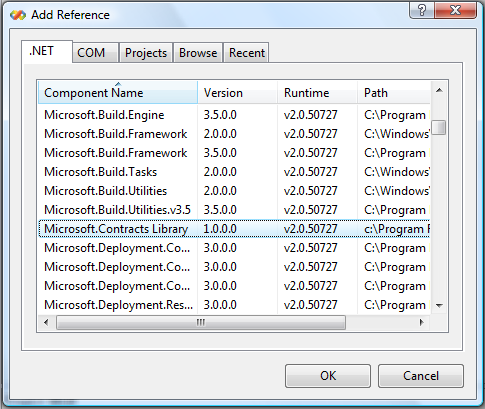
\includegraphics[width=.7\columnwidth]{../Common/addRef.png}
\end{center}



\section{Sample Walkthrough}
\label{sec:start}

After adding the proper reference, go to the Properties of project
\textsf{\ProjectName}, select the Code Contracts pane (at the bottom), and enable static checking by clicking on the static checking box. 
Also enable implicit non-null, array checks, container analysis and caching as shown in this screenshot:
\begin{center}
  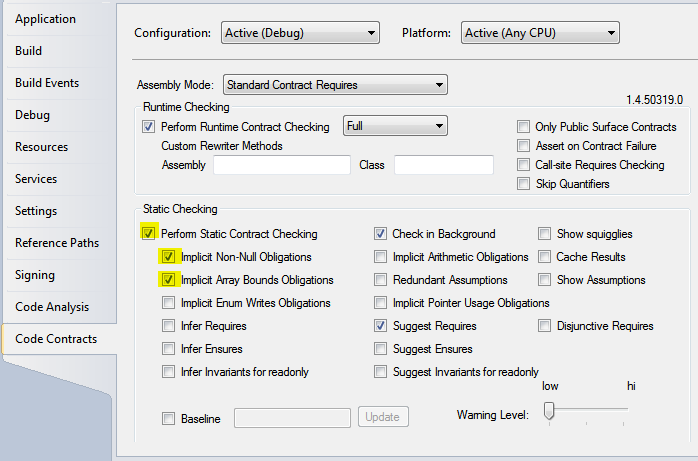
\includegraphics[width=.8\columnwidth]{ex1.png}
\end{center}

Then build the example. The build should succeed. After a
moment\footnote{The static checker runs in the background after the regular build.}, 
the static checker should warn about the following problems:
\begin{center}
  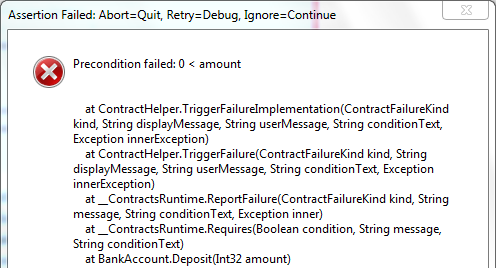
\includegraphics[width=1\columnwidth]{ex2.png}
\end{center}
The first warning is orginated by the fact that the static checker is missing the information that all the array elements of indexes \code{0} \dots \code{index} are not null.
We can make this information explicit  by adding the following object invariant (in the example, just uncomment it):
\begin{lstlisting}
  Contract.Invariant(Contract.ForAll(0, nextFree, i => arr[i] != null));
\end{lstlisting}
If we build again, we notice that the number of checked assertions as increased.
This is due to the fact that now also the condition on the elements of \code{arr} is checked at method exits.
\begin{center}
  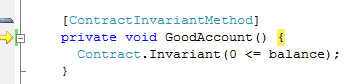
\includegraphics[width=1\columnwidth]{ex3.png}
\end{center}
We are left with the last message from the static checker, warning us that the array access may be not be in bounds.
This happens when \code{arr.Length} is zero.
Changing the array creation expression as 
\begin{lstlisting}
  var newArr = new T[arr.Length * 2 + 1];
\end{lstlisting}
solves the problem:
\begin{center}
  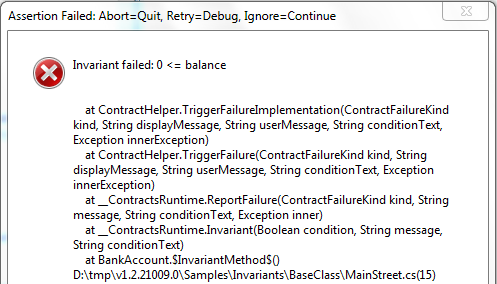
\includegraphics[width=1\columnwidth]{ex4.png}
\end{center}
\code{Push} was the only  modified method, so the checker used the cache to avoid re-analyzing the unmodified methods (Properties are not cached):

\begin{verbatim}
CodeContracts: NonNullStack: Total methods analyzed 6
CodeContracts: NonNullStack: Total method analysis read from the cache 3
\end{verbatim}


\end{document}
